\documentclass[journal]{IEEEtran}
\usepackage[T1]{fontenc}
\usepackage[utf8]{inputenc}
\usepackage{amsmath,amssymb,amsthm}
\usepackage{booktabs}
\usepackage{graphicx}
\usepackage{xcolor}
\usepackage{url}
\usepackage{algorithm}
\usepackage{algpseudocode}
\newtheorem{proposition}{Proposition}
\newcommand{\sys}{\textsc{Dots}}
\usepackage{cite}
\let\citep\cite \let\citet\cite
\usepackage[hidelinks]{hyperref}
\begin{document}
\title{DOTS: Exactly Removable Continual Learning for Frozen Language Models via Hyperdimensional Sparse Memory}
\author{Sohan Merugu\thanks{S. Merugu is an independent researcher (e-mail: sohanmerugu@gmail.com).}}
\markboth{S. Merugu: DOTS}{S. Merugu: DOTS}
\maketitle
\begin{abstract}
A language model that keeps learning after deployment must also be able to forget on request. We present \sys{}, a retrofit that attaches a 262{,}144-slot sparse memory to a frozen pretrained transformer and records every learned unit of knowledge, a \emph{Dot}, in a ledger. Memory addresses are fixed random hypervectors applied to whitened hidden states, so attaching the memory leaves the model's outputs bit-identical and a learned item is never orphaned by address drift. Each Dot writes only value rows that ordinary text rarely reads and that no earlier Dot owns, using a per-Dot optimizer under deterministic kernels. Because every Dot logs the slots it read and wrote, removing a Dot reduces to restoring rows and replaying only the Dots it could have influenced. The result is bitwise identical to a model that never learned the removed Dot. On Qwen2.5-0.5B learning 1{,}000 TriviaQA facts it did not know, in ten sequential Dots, \sys{} recalls 96.1\% of the facts (73.5\% under a prompt context never seen in training), keeps 86.3\% of facts the model already knew, and changes held-out perplexity by 1.6\%. The best full fine-tuning run keeps 51.3\% of known facts and the best LoRA run 33.0\%. We verify bit-exact removal and reset on both CPU and GPU, and we report the main cost: in our setting every removal replays all later Dots.
\end{abstract}
\begin{IEEEkeywords}
Continual learning, machine unlearning, sparse memory, large language models, catastrophic forgetting, hyperdimensional computing.
\end{IEEEkeywords}


\section{Introduction}

Deployed language models are frozen. A model that could keep learning from the documents its user chooses, on the user's own machine, would need two properties that pull against each other. It must write new knowledge into its parameters without erasing what it already knows, and it must be able to take any piece of that knowledge back out. Dense weight updates fail the first property \citep{mccloskey1989,kirkpatrick2017ewc,ibrahim2024simple}. Approximate unlearning fails the second: knowledge suppressed by gradient-based unlearning returns after 4-bit quantization, from roughly 21\% to 83\% retained \citep{zhang2025quant}.

Sparse memory layers point toward a way to satisfy both. Product-key memories add millions of key-value slots of which each token reads only a few \citep{lample2019pkm,berges2024memory}. Updating only the slots that new data uses more than background data does strongly reduces forgetting \citep{lin2025smf,goyal2026improving,gupta2026smf}. Exact removal, however, needs more than sparsity. Every later update was computed in the presence of earlier ones, so subtracting a logged parameter delta does not recover the state a model would have had without that data. Exact deletion in the literature comes from isolation by design and deterministic replay \citep{bourtoule2021sisa,x2025trace,kuo2025sift}.

\sys{} combines these lines of work into one mechanism. Its contributions are:

\begin{enumerate}
  \item \textbf{A training-free retrofit.} A sparse memory is attached in parallel to one MLP block of a frozen model. Addressing uses a fixed random projection of whitened hidden states and fixed random bipolar sub-keys, so nothing in the address path is trained and attaching the memory changes no output bit (\S\ref{sec:retrofit}).
  \item \textbf{A write rule for low interference.} Each Dot selects slots by TF-IDF against background usage, never writes slots that ordinary text reads heavily or that earlier Dots own, and trains only those rows (\S\ref{sec:write}).
  \item \textbf{A ledger with exact removal.} Dots log read and write sets. We state the conditions under which dropping a Dot and replaying its taint closure is bitwise equal to never having learned it, and verify this on CPU and on GPU (\S\ref{sec:ledger}, \S\ref{sec:removal}).
  \item \textbf{An empirical comparison} on Qwen2.5-0.5B against tuned LoRA and full fine-tuning, including recall under an unseen prompt context and the removal cost (\S\ref{sec:results}).
\end{enumerate}

\section{Related Work}

\paragraph{Sparse memory layers.} Product-key memory \citep{lample2019pkm} and its scaled versions \citep{berges2024memory} replace or augment feed-forward blocks with large key-value tables. Sparse memory finetuning \citep{lin2025smf} updates only the value rows most specific to new data relative to background batches. On a 1.3B model learning 1{,}000 facts it reduced the NaturalQuestions F1 drop from 89\% (full fine-tuning) and 71\% (LoRA) to 11\%. Retrofits into Qwen2.5-0.5B followed \citep{goyal2026improving,gupta2026smf}. Hierarchical memory banks separate long-tail knowledge from a small core model and allow memory blocks to be deleted \citep{pouransari2026hier}. \sys{} differs in that its memory is added to an unchanged model without any further training, its addresses are fixed rather than learned, and every write is logged so that removal is exact rather than approximate.

\paragraph{Test-time training and fast weights.} Fast-weight programmers update a matrix state with each token \citep{schlag2021linear}. Gated delta rules \citep{yang2025gated}, test-time training layers \citep{sun2024ttt}, Titans \citep{behrouz2025titans}, and nested learning \citep{behrouz2025nested} treat parts of the network as memories trained during inference. In-place test-time training updates a pretrained model's own MLP projections \citep{feng2026inplace}, and fast-weight product-key memory applies such updates to sparse slots \citep{zhao2026fwpkm}. These methods target in-context adaptation and reset their state at document or request boundaries. \sys{} targets persistent knowledge and its reversal.

\paragraph{Knowledge editing.} Locate-and-edit methods change MLP weights from (subject, relation, object) triples \citep{meng2022rome,meng2023memit,fang2025alphaedit}. Codebook editors store edits in separate key-value entries \citep{hartvigsen2023grace,wang2024wise}. Larimar writes to an episodic memory in closed form and removes an entry with the same update \citep{das2024larimar}. MemoryLLM keeps a self-updating latent memory pool \citep{wang2024memoryllm}. \sys{} learns from ordinary question-answer text rather than triples and keeps its writes addressable for removal.

\paragraph{Continual learning and forgetting.} Catastrophic interference \citep{mccloskey1989} is commonly reduced by regularizing important weights \citep{kirkpatrick2017ewc} or replaying earlier data \citep{ibrahim2024simple}. LoRA \citep{hu2022lora} learns less and also forgets less than full fine-tuning \citep{biderman2024lora}. Long training sequences also erode plasticity \citep{dohare2024loss}. Dynamic evaluation finds that resetting online updates at document boundaries works best \citep{rannentriki2024dynamic}, which is evidence against naive always-on full-weight learning.

\paragraph{Machine unlearning.} Approximate methods such as negative preference optimization \citep{zhang2024npo} suppress outputs but can be undone \citep{zhang2025quant}. Exact methods isolate data at training time: SISA retrains only the affected shard \citep{bourtoule2021sisa}, SIFT-Masks merges and unmerges sign-constrained finetunes \citep{kuo2025sift}, and deterministic replay reproduces deletion counterfactuals bit for bit at 1--2.8B scale \citep{x2025trace}. Gradient routing and selective gradient masking localize a capability so it can be zeroed \citep{cloud2024gradient,shilov2025sgtm}. FlexOlmo and NULLs isolate data sources architecturally \citep{shi2025flexolmo,ghosal2026nulls}. \sys{} applies isolation and replay at the granularity of memory rows, with a dependency analysis that decides which Dots must be replayed.

\paragraph{Hyperdimensional computing.} Vector-symbolic architectures compute with quasi-orthogonal random high-dimensional vectors \citep{plate1995hrr,kanerva2009hdc}. Sparse distributed memory \citep{kanerva1988sdm} stores data at many hard locations addressed by similarity, and attention approximates it \citep{bricken2021attention}. The capacity of a single superposition vector grows only linearly with dimension \citep{frady2018theory}, which motivates storing knowledge across many slots instead. Random sign projections preserve angles \citep{charikar2002simhash}, and open tooling for these operations exists \citep{heddes2023torchhd}. We use these ideas only for addressing: fixed random sub-keys and a fixed random projection.

\section{Method}

\subsection{Retrofitting a sparse memory}
\label{sec:retrofit}

Let $x \in \mathbb{R}^{d}$ be the input to the MLP of decoder layer $\ell$ (the output of its post-attention normalization). \sys{} replaces the block's MLP output $\mathrm{MLP}(x)$ with $\mathrm{MLP}(x) + M(x)$, where $M$ is a sparse memory with $N = S^2$ slots and value table $V \in \mathbb{R}^{N \times d}$.

\paragraph{Addressing.} The input is whitened with background statistics, $z = (x-\mu)\oslash\sigma$, and projected by a fixed Gaussian matrix $P \in \mathbb{R}^{d\times 2k}$ with entries $\mathcal{N}(0, 1/d)$. The result $q = zP$ is split into halves $q_1, q_2 \in \mathbb{R}^{k}$. Each half is matched against $S$ fixed random bipolar sub-keys $K_1, K_2 \in \{-1,+1\}^{S\times k}$, with scores $s_j = q_j K_j^\top/\sqrt{k}$. As in product-key memory \citep{lample2019pkm}, the top-$t$ candidates from each half are combined into $t^2$ slot candidates with score $s_1[a]+s_2[b]$ and slot index $aS+b$. The top-$t$ of these are read with weights $w = \mathrm{softmax}(\text{score}/\tau)$:
\begin{equation}
M(x) = \sum_{i \in \mathrm{top}\text{-}t(x)} w_i\, V_i .
\end{equation}
$P$, $K_1$ and $K_2$ are drawn once from a seeded generator and never trained. A slot's address therefore depends only on the frozen model and the input, and does not drift as learning proceeds.

\paragraph{Function preservation.} $V$ starts at zero, so $\mathrm{MLP}(x) + M(x) = \mathrm{MLP}(x)$ exactly and the retrofitted model's outputs are bit-identical to the original's. We verify this on every run.

\paragraph{Calibration.} Two background statistics are computed with forward passes only. The first is the whitening mean and standard deviation $(\mu, \sigma)$. The second is, for every slot, its document frequency $\mathrm{df}_i$ (how many background sequences read it) and its read mass $m_i$ (the sum of read weights). The background mixes plain text with text in the format the model will be queried in (\S\ref{sec:setup}). This mix matters: with plain text only, slots read by the question-answer format itself look rare and are selected for writing, which damages unrelated questions (Table~\ref{tab:ablation}).

\subsection{Writing a Dot}
\label{sec:write}

A Dot is one batch of training examples from one source, here 100 question-answer facts. Learning a Dot proceeds as follows (Algorithm~\ref{alg:write}).

\begin{enumerate}
  \item \textbf{Cache.} Run layers $<\ell$ once and cache their output. Layers below the memory never change, so training needs forward and backward passes only through layers $\geq\ell$.
  \item \textbf{Read set.} Record every slot the Dot's tokens read, $R$, and per-slot read counts $c_i$.
  \item \textbf{Select.} Score each read slot by $c_i \log\frac{D+1}{\mathrm{df}_i+1}$, where $D$ is the number of background sequences. Exclude slots whose read mass $m_i$ lies above the 90th percentile of all slots (\emph{protection}) and slots written by earlier Dots (\emph{ownership}). Keep the top $B$ slots as the write set $W$.
  \item \textbf{Train.} Optimize only the rows $V_W$ with a fresh Adam optimizer \citep{kingma2015adam} on the next-token loss over answer tokens. Minibatch order comes from a seed derived from a hash of the Dot's data.
  \item \textbf{Log.} Store the delta $\Delta = V_W^{\text{after}} - V_W^{\text{before}}$ together with $W$, $R$, the seed, the source, and the training examples.
\end{enumerate}

All other parameters, including the address path, stay frozen. Training runs with PyTorch's deterministic algorithms enabled \citep{pytorchrepro} and a cross-entropy computed from log-softmax and one-hot targets, which avoids atomic additions on GPU. Without deterministic algorithms, two CPU runs of the same Dot differed by up to $1.1\times10^{-4}$ in the learned rows, enough to break bit-exact replay.

\begin{algorithm}[t]
\caption{Learning a Dot and recording it in the ledger}
\label{alg:write}
\begin{algorithmic}[1]
\Require frozen model with memory at layer $\ell$; ledger $\mathcal{L}$ with Dots $d_1..d_n$; examples $E$
\State $V \gets \textsc{Materialize}(\mathcal{L})$ \Comment{$V = V_0 + \sum_j \Delta_j$ in Dot order}
\State $h \gets$ layers$_{<\ell}(E)$; \; $(R, c) \gets$ reads of $E$ at layer $\ell$
\State $O \gets \bigcup_j W_j$ \Comment{slots owned by earlier Dots}
\State $W \gets \mathrm{top}\text{-}B\{\, c_i \log\frac{D+1}{\mathrm{df}_i+1} : i \in R \setminus O,\ m_i \le q_{0.9}(m) \,\}$
\State $\theta \gets V_W$; optimize $\theta$ with fresh Adam, seed $\mathrm{hash}(E)$, deterministic kernels
\State append $d_{n+1} = (W, R, \Delta = \theta - V_W, \mathrm{seed}, E)$ to $\mathcal{L}$; \Return $\textsc{Materialize}(\mathcal{L})$
\end{algorithmic}
\end{algorithm}

\subsection{The ledger: reset and exact removal}
\label{sec:ledger}

The canonical memory state is $V = V_0 + \sum_{j} \Delta_j$, summed in Dot order over each Dot's write rows. It is always recomputed from the deltas, never obtained by subtraction, because floating-point addition is not invertible. \textbf{Reset} drops all Dots and restores $V_0$, which is zero after a retrofit.

\textbf{Removal} of Dot $k$ first computes its \emph{taint closure} $T$. Process Dots after $k$ in order, starting from a tainted slot set $\mathcal{T} = W_k$. A Dot $j$ is tainted if $R_j \cap \mathcal{T} \neq \emptyset$, and a tainted Dot adds $W_j$ to $\mathcal{T}$. Removal then drops $d_k$ and walks the remaining Dots in order. Untainted Dots keep their deltas. Each tainted Dot is replayed from its logged data and seed on the state materialized from the Dots kept before it, recomputing its slot selection.

\begin{proposition}
\label{prop:exact}
Assume (i) the model and the address path are frozen; (ii) a Dot's training reads only the rows in its read set, and its optimizer state does not outlive it; (iii) slot selection depends only on the Dot's data, the frozen background statistics, and the owned slots inside its read set; and (iv) execution is deterministic. Then the state after removing Dot $k$ by taint-closure replay is bitwise identical to the state obtained by learning the remaining Dots, in order, from $V_0$.
\end{proposition}

\noindent\emph{Proof sketch.} Induct over the Dots after $k$. For an untainted Dot $j$, every row in $R_j$ has the same value in both histories, because rows in $R_j$ were written either by untainted Dots, whose deltas are identical by induction, or by no Dot. Its owned set inside $R_j$ is also identical, so by (ii)--(iv) its selection, gradients and delta are identical. For a tainted Dot, both histories replay the same data and seed from the same materialized state, so they agree by (iv). It remains to check that a replayed Dot cannot write a slot outside $\mathcal{T}$ that an untainted Dot reads. A replayed Dot's eligible set differs from the original only by slots that the removed or replayed Dots previously owned, and with a fixed budget its new top-$B$ set lies inside its old write set together with those freed slots. All of these are in $\mathcal{T}$. $\square$

\textbf{Fast removal} drops $\Delta_k$ without replay. It is instant but not exact when later Dots read $W_k$. We measure both.

\subsection{Context augmentation}
\label{sec:aug}

A Dot trained only on the plain prompt \texttt{Question: q\textbackslash nAnswer:} is addressed through hidden states that depend on the whole context. When the same question is preceded by demonstrations, different slots are read and recall drops (\S\ref{sec:results}). \sys{} v2 therefore trains each fact in three contexts: the plain prompt and two demonstration prefixes (a two-shot and a three-shot prefix, listed in Appendix~\ref{app:prompts}). Evaluation uses a third demonstration prefix that never appears in training.

\section{Experimental Setup}
\label{sec:setup}

\paragraph{Model and memory.} We retrofit Qwen2.5-0.5B \citep{qwen2025} (24 layers, $d=896$) in fp32 at layer $\ell=15$, with $S=512$ ($N=262{,}144$ slots), $k=128$, $t=32$ and $\tau=1$. The value table holds 235M parameters (0.94\,GB in fp32).

\paragraph{Calibration data.} The background consists of 400 WikiText-2 training chunks of 128 tokens \citep{merity2017wikitext} and 1{,}500 NaturalQuestions-open \emph{training} question-answer pairs \citep{kwiatkowski2019nq,lee2019orqa}. Of these pairs, 1{,}000 are in the plain format and 500 carry the evaluation demonstration prefix. Whitening statistics come from the first 12 mixed batches.

\paragraph{Facts.} From TriviaQA \citep{joshi2017triviaqa} (rc.nocontext) we keep questions with answers of at most three words. The base model is evaluated with greedy decoding under a three-shot prefix. We take 1{,}000 training-split questions it answers \emph{incorrectly} (base exact match on the candidates: 20.6\%) as facts to learn. We take 300 validation-split questions it answers \emph{correctly} as \emph{known facts}, a retention probe. The facts to learn are split into ten Dots of 100, learned in sequence.

\paragraph{Metrics.} We report: \emph{taught EM}, exact match on all 1{,}000 learned facts in the training format; \emph{unseen-context EM}, exact match on the first 200 learned facts under the held-out three-shot prefix; \emph{known kept}, exact match on the 300 known facts under the same prefix (100\% for the base model by construction); NaturalQuestions-open F1 on 300 validation questions; and perplexity on 12{,}800 WikiText-2 test tokens.

\paragraph{\sys{} settings.} Adam with learning rate 0.03 and batch size 16. v1 uses 120 steps and $B=3{,}000$ write slots per Dot. v2 uses 240 steps and $B=6{,}000$, because each Dot holds three contexts per fact. These settings were chosen in single-Dot sweeps as the configuration with the highest recall that kept at least 97\% of a 100-fact known subset (Table~\ref{tab:ablation}).

\paragraph{Baselines.} \emph{Full fine-tuning} updates all 358M non-embedding parameters with Adafactor \citep{shazeer2018adafactor}; the tied embedding matrix is frozen to fit memory. \emph{LoRA} \citep{hu2022lora} uses rank 32 and $\alpha=64$ on all attention and MLP projections (17.6M parameters) with AdamW. Both see the same ten chunks in the same order, with the same answer-only loss, batch size 16 and 60 steps per chunk. The variants marked +aug use the v2 context-augmented data and 120 steps. We sweep three learning rates for each baseline. All baseline runs except LoRA at $3\times10^{-5}$ (77\%) reach 98--100\% recall on a chunk immediately after training on it (Table~\ref{tab:main}), so their acquisition is not limited by the step budget.

\paragraph{Hardware and reproducibility.} Main results come from a free Colab NVIDIA T4 GPU. The v1 pipeline was also run on a 6-core laptop CPU (Intel i7-9750H, 8\,GB RAM). All runs are single executions. \sys{} training is deterministic, and two independent T4 runs of v1 produced identical metrics.

\section{Results}
\label{sec:results}

\begin{table*}[t]
\centering
\small
\caption{Learning 1{,}000 unknown TriviaQA facts as ten sequential Dots on Qwen2.5-0.5B (T4 GPU). ``After'' is recall of the first chunk immediately after it was learned. Base model: NQ EM 5.7, NQ F1 9.9, perplexity 27.43.}
\label{tab:main}
\begin{tabular}{lcccccc}
\toprule
Method & Taught & Unseen ctx. & Known kept & NQ F1 & PPL & After \\
\midrule
\sys{} v2 (augmented) & \textbf{96.1} & \textbf{73.5} & 86.3 & 9.2 & 27.88 & 94 \\
\sys{} v1 & 91.5 & 10.5 & \textbf{91.3} & \textbf{10.3} & \textbf{27.75} & 95 \\
\midrule
Full FT, lr $5\!\times\!10^{-6}$ & 82.3 & 51.0 & 51.3 & 6.9 & 31.66 & 99 \\
Full FT, lr $1\!\times\!10^{-5}$ & 83.7 & 52.0 & 39.3 & 6.1 & 35.65 & 100 \\
Full FT, lr $2\!\times\!10^{-5}$ & 83.8 & 46.5 & 25.7 & 2.8 & 46.77 & 100 \\
Full FT, lr $1\!\times\!10^{-5}$ +aug & 84.7 & 61.0 & 43.0 & 4.9 & 35.80 & 100 \\
\midrule
LoRA, lr $3\!\times\!10^{-5}$ & 49.2 & 16.5 & 27.7 & 5.4 & 39.28 & 77 \\
LoRA, lr $1\!\times\!10^{-4}$ & 53.0 & 26.5 & 29.7 & 2.7 & 45.09 & 98 \\
LoRA, lr $3\!\times\!10^{-4}$ & 37.4 & 3.5 & 6.3 & 0.0 & 134.57 & 100 \\
LoRA, lr $1\!\times\!10^{-4}$ +aug & 57.9 & 22.0 & 33.0 & 4.8 & 47.72 & 100 \\
\bottomrule
\end{tabular}
\end{table*}

\paragraph{Learning without forgetting.} Table~\ref{tab:main} and Figure~\ref{fig:tradeoff} summarize the comparison. \sys{} v1 learns 91.5\% of the 1{,}000 facts while keeping 91.3\% of the known facts. NQ-open F1 (10.3 against 9.9 for the base model) and perplexity (+1.1\%) are essentially unchanged. The best full fine-tuning run keeps 51.3\% of known facts, with NQ F1 falling to 6.9 and perplexity rising 15\%. LoRA keeps at most 33.0\%. Sparse writes also avoid interference among new facts. Figure~\ref{fig:perdot} shows recall of each Dot after all ten were learned. Under \sys{} the first Dot stays at 96\%, while full fine-tuning and LoRA show a recency curve, with the first chunk at 62\% and 28\% respectively.

\begin{figure*}[t]
\centering
\begin{minipage}[t]{0.48\textwidth}
\centering
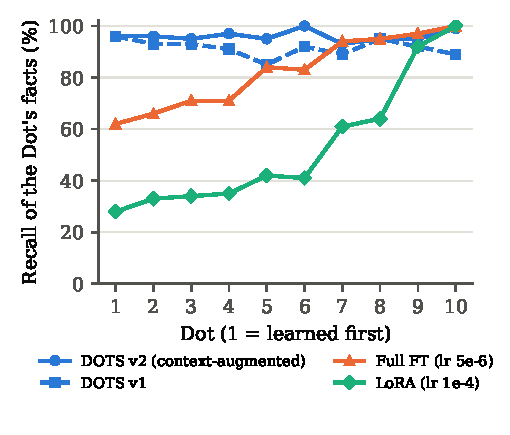
\includegraphics[width=\linewidth]{figures/per_dot_recall.pdf}
\caption{Recall of each Dot's facts after all ten Dots were learned. Baselines forget earlier chunks; \sys{} does not.}
\label{fig:perdot}
\end{minipage}\hfill
\begin{minipage}[t]{0.48\textwidth}
\centering
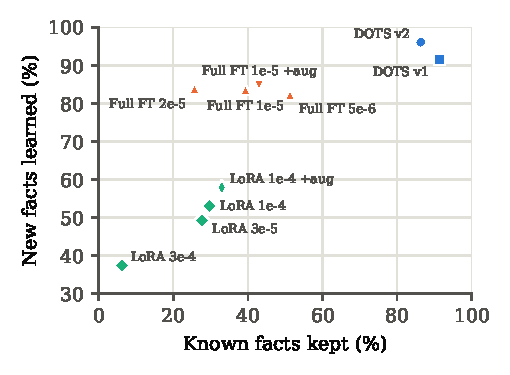
\includegraphics[width=\linewidth]{figures/tradeoff.pdf}
\caption{New facts learned against known facts kept, for every run in Table~\ref{tab:main}.}
\label{fig:tradeoff}
\end{minipage}
\end{figure*}

\paragraph{Context generalization.} \sys{} v1 recalls taught facts in the training format (91.5\%) but only 10.5\% of them when the question follows an unseen three-shot prefix, below full fine-tuning (51.0\%). The memory is addressed through context-dependent hidden states, and v1 trained only one context. Training each fact in two additional contexts (v2) raises unseen-context recall to 73.5\%, above every baseline, including full fine-tuning on the same augmented data (61.0\%). The cost is retention: known facts kept falls from 91.3\% to 86.3\%, because v2 writes twice as many rows.

\subsection{Removal and reset}
\label{sec:removal}

\begin{table*}[t]
\centering
\small
\caption{Removing Dot 1 after all ten Dots were learned (T4 GPU). ``Equal to never learned'' compares the full value table bitwise with a model that learned only Dots 2--10.}
\label{tab:removal}
\begin{tabular}{llcccc}
\toprule
Version & Operation & Dot 1 EM & Dot 2 EM & Known kept & Time \\
\midrule
v1 & before removal & 96 & 93 & 91.3 & -- \\
v1 & fast (drop $\Delta_1$) & 3 & 57 & 93.7 & $<$0.1\,s \\
v1 & exact (replay 9 Dots) & 6 & 97 & 92.3 & 194\,s \\
v2 & fast (drop $\Delta_1$) & 4 & 58 & 90.3 & $<$0.1\,s \\
v2 & exact (replay 9 Dots) & 6 & 98 & 87.3 & 718\,s \\
\midrule
\multicolumn{6}{l}{Exact removal equal to never learned: \textbf{yes} (v1 and v2, T4; v1 on CPU and in a 3-Dot smoke test)} \\
\multicolumn{6}{l}{Reset: value-table hash and output logits equal to the original model: \textbf{yes}} \\
\bottomrule
\end{tabular}
\end{table*}

Table~\ref{tab:removal} reports removal of the first Dot. Exact removal produced a value table bitwise identical to a model that learned only Dots 2--10, in every configuration we ran: v1 and v2 on the T4 GPU and v1 on the laptop CPU. Recall of the removed facts falls to 6\%. This equals the never-learned model, which answers 6\% of them, presumably because some facts can be inferred from facts in other Dots. Dot 2's recall is 97--98\% after replay.

Fast removal is instant but damages later Dots: Dot 2 falls from 93\% to 57\%, because Dot 2 was learned while Dot 1's rows were present. Reset restores a value table whose hash, and the model's output logits, equal the original model's.

\paragraph{Fan-out.} Every Dot read at least one slot written by every earlier Dot, so removing Dot $k$ replays all later Dots. The fan-out was 100\% in both versions. Removal cost is therefore linear in the number of later Dots: 194\,s for nine Dots on the T4 for v1, and 3{,}247\,s on the laptop CPU. This is the main open problem (\S\ref{sec:limits}).

\subsection{What makes writes safe}

\begin{table*}[t]
\centering
\small
\caption{Single-Dot ablations on CPU (100 facts learned; 100 known facts). Rows are cumulative unless noted.}
\label{tab:ablation}
\begin{tabular}{lcc}
\toprule
Write policy & Learned & Known kept \\
\midrule
SGD, lr 2--32, WikiText background & 2--4 & 93--100 \\
Adam, lr 0.03, WikiText background & 92 & 77 \\
\quad + Q\&A-format background & 90 & 87 \\
\quad + read-mass protection (top 10\%) & 57 & 98 \\
\quad + protection, lr 0.06 & 91 & 96 \\
\quad + protection, 120 steps (selected) & \textbf{95} & \textbf{99} \\
\midrule
anchor penalty instead of protection & 58 & 95 \\
protection + anchor penalty & 38 & 100 \\
memory at layer 19 (Adam 0.03, WikiText background) & 56 & 79 \\
budget $B=1{,}000$ (Adam 0.03, Q\&A background) & 48 & 96 \\
\bottomrule
\end{tabular}
\end{table*}

Table~\ref{tab:ablation} isolates the components. Plain SGD barely moves the memory: the residual stream at layer 15 is large relative to the updated rows, and Adam's normalized steps are needed. Background statistics drawn only from plain text leave the question-answer format's own slots looking rare, so writes land on slots that every question reads. Adding Q\&A-format text to the background raises known-fact retention from 77\% to 87\%. Excluding the 10\% of slots with the highest background read mass raises it to 98\%; more steps then recover acquisition. In the earlier synthetic-memory prototype (Appendix~\ref{app:proto}), ownership stopped new Dots from overwriting older ones. In the full ten-Dot runs here, earlier Dots also keep their recall (Figure~\ref{fig:perdot}).

\paragraph{Cost.} A v1 Dot of 100 facts took about 21\,s on the T4 and 380\,s on the laptop CPU. The ledger stored 10.3\,MiB per Dot for v1 and 20.6\,MiB for v2. Most of this is the logged deltas, which can be recomputed from the logged text when space matters.

\section{Limitations}
\label{sec:limits}

\begin{itemize}
  \item \textbf{Scale and scope.} One 0.5B model, one memory layer and one dataset of short factual answers. We do not show that memory writes can teach skills or longer documents. A 2026 retrofit study reported only small task gains from sparse memory finetuning \citep{gupta2026smf}.
  \item \textbf{Removal cost.} With 100\% fan-out, exact removal replays every later Dot. Reducing fan-out, for example by restricting a Dot's reads during training to a source-specific shard of slots, or by keeping periodic snapshots, is future work.
  \item \textbf{Retention trade-off.} Context augmentation improves generalization but lowers known-fact retention from 91.3\% to 86.3\%.
  \item \textbf{Baselines.} We swept three learning rates per baseline at a fixed step budget. Other schedules, replay, or regularization might change their retention. \sys{} also used more steps per Dot (120 or 240) than the baselines (60 or 120).
  \item \textbf{Statistics.} All results are single runs. \sys{} is deterministic given the data order, but we did not vary data order, fact sets, or the memory's random seed.
  \item \textbf{Exactness boundary.} Proposition~\ref{prop:exact} covers knowledge written by Dots. Knowledge from pretraining is not removable by this mechanism, and facts the model can re-derive from remaining Dots are not leakage.
\end{itemize}

\section{Broader Impact}

A model that keeps learning on a user's device learns whatever it is given, including false or harmful material. Small numbers of poisoned documents can backdoor models regardless of size \citep{souly2025poisoning}. A per-source ledger helps here: any source can be audited and exactly removed. It also supports data-deletion requests, which approximate unlearning cannot reliably meet \citep{zhang2025quant}. Sharing Dots between users would make users distributors of what the Dots encode. Model-weight versioning systems such as Git-Theta \citep{kandpal2023gittheta} show how such sharing could be tracked.

\section{Conclusion}

\sys{} retrofits a frozen language model with a sparse memory whose fixed hyperdimensional addresses, protected and owned write sets, and deterministic per-Dot training make continual factual learning both low-interference and exactly reversible. On Qwen2.5-0.5B it learns 96.1\% of 1{,}000 new facts while keeping 86.3\% of known facts, compared with at most 51.3\% for tuned full fine-tuning. Removing any Dot yields a model bitwise identical to one that never learned it. The open problems are removal cost under full fan-out and evidence at larger scale and beyond facts.

\section*{Code and Data Availability}
The code (retrofit, writer, ledger, evaluation and the self-contained Colab notebooks) and the exact fact lists will be released at \url{https://github.com/sohan-a11y/open-dots}. All data come from public datasets: TriviaQA, NaturalQuestions-open and WikiText-2.

\section*{Use of AI Assistance}
An AI system (Claude, Anthropic) assisted with literature search, code, experiment design iterations and drafting of this manuscript. The author reviewed all content and takes full responsibility for it.

\section*{Author Contributions, Conflicts of Interest and Funding}
S.M.: conceptualization, investigation, writing (review and editing). The author declares no competing interests. This work received no external funding.

\bibliographystyle{IEEEtran}
\bibliography{references}

\appendix
\section{Prompts}
\label{app:prompts}
Training and plain-format evaluation use \texttt{Question: \{q\}\textbackslash nAnswer:} with target \texttt{ \{a\}\textbackslash n}; loss is on target tokens only.
Training prefix A (two-shot): gold $\rightarrow$ Au; largest ocean $\rightarrow$ Pacific Ocean.
Training prefix B (three-shot): inventor of the telephone $\rightarrow$ Alexander Graham Bell; tallest mountain $\rightarrow$ Mount Everest; legs of a spider $\rightarrow$ 8.
Held-out evaluation prefix (three-shot, never trained): capital of Japan $\rightarrow$ Tokyo; Red Planet $\rightarrow$ Mars; painter of the Mona Lisa $\rightarrow$ Leonardo da Vinci.

\section{Hyperparameters}
\noindent\begin{tabular}{@{}lp{0.78\linewidth}@{}}
\toprule
Memory & layer 15; $S=512$ ($N=262{,}144$); $k=128$; $t=32$; $\tau=1$; values zero-initialized \\
Calibration & 400$\times$128 WikiText-2 tokens + 1{,}500 NQ-open train Q\&A; stats from 12 batches \\
\sys{} v1 & Adam 0.03; 120 steps; batch 16; $B=3{,}000$; protection at the 90th percentile \\
\sys{} v2 & as v1 with 240 steps, $B=6{,}000$, three contexts per fact \\
Full FT & Adafactor; lr $\{5\!\times\!10^{-6}, 10^{-5}, 2\!\times\!10^{-5}\}$; 60 steps per chunk; embeddings frozen \\
LoRA & $r=32$, $\alpha=64$, all projections; AdamW; lr $\{3\!\times\!10^{-5}, 10^{-4}, 3\!\times\!10^{-4}\}$; 60 steps \\
Determinism & deterministic PyTorch algorithms; cuBLAS workspace \texttt{:4096:8}; eager attention on GPU \\
\bottomrule
\end{tabular}

\section{Synthetic prototype}
\label{app:proto}
Before the retrofit, we tested the same mechanisms in a 2.6M-parameter byte-level model trained from scratch. It had an attention block, a gated delta-rule fast-weight block, and a 16{,}384-slot memory with fixed bipolar sub-keys. It was trained on 400 fictional entities and then learned two sets of 100 new entities. Full fine-tuning kept 12.4\% of the original facts after two rounds. The \sys{} write policy kept 93\%, and 100\% with a 65{,}536-slot memory. Slot ownership kept the first new set at 50\% after the second was learned, against 28.5\% without ownership. Exact removal and reset were bitwise exact.

\end{document}
